% this is a comment in latex
% substitute this documentclass definition for uncommented one
% to switch between single and double column mode
\documentclass[11pt,twocolumn]{article}
%\documentclass[11pt]{article}

\usepackage{fullpage}
\usepackage{subfigure,indentfirst}
% for url
\usepackage{hyperref}
% for underlined text
\usepackage[normalem]{ulem}
% for including pdf figures
\usepackage{graphicx}
\usepackage{float}

% my own versions: my_enumerate and my_itemize
\newenvironment{my_enumerate}{
  \begin{enumerate}
    \setlength{\itemsep}{1pt}
      \setlength{\parskip}{0pt}
\setlength{\parsep}{0pt}}{\end{enumerate}
}

\newenvironment{my_itemize}{
  \begin{itemize}
    \setlength{\itemsep}{1pt}
      \setlength{\parskip}{0pt}
\setlength{\parsep}{0pt}}{\end{itemize}
}

% this starts the document
\begin{document}

\title{Reduct, Deduplicated Distributed File System}

\author{Keonwoo Oh, Sam Rothstein, Ford Johnstone \\
Computer Science Department, Swarthmore College, Swarthmore, PA  19081}

\maketitle

\begin{abstract}

We designed, implemented, and tested Reduct, a deduplicated distributed file system. Our motivation for designing a new system stemmed from an observation of numerous shortcomings in the existing distributed file systems, including excessive metadata and the possibility of data corruption due to hash collisions. Our solution is closely modeled after widely used distributed file systems such as the Google File System and HDFS (Hadoop Distributed File System), yet internally supports subfile level deduplication in a way that avoids the aforementioned issues. 

Several experiments were conducted to test the performance of Reduct in terms of deduplication ratio, read, and write speeds. The primary focus was to measure not only the effectiveness of deduplication, but also its impact on the throughput of the system. Our experimental results were positive, despite the various limitations of the project due to time constraint. Future research would require implementing and testing a full-scale system that is far more reliable and efficient. 
\end{abstract}


\section {Introduction} 

With the tremendous influx of data, there is an ever increasing need to take measures to reduce data storage, yet maintain data integrity. Data deduplication and data compression are the two main methods for conserving data storage. Data deduplication refers to the elimination of redundant data while data compression refers to the process of encoding information using fewer bits\cite{Overview}. Given that many files consist of duplicates and that duplicates take up space at the file level, data deduplication could effectively reduce data storage. Data deduplication would be particularly effective in a distributed file system that contains large amount of data with many duplicates\cite{Overview}.

Conventional distributed file systems such as the HDFS (Hadoop Distributed File System), and Google File System do not have innate support for deduplication\cite{GFS}\cite{HDFS}. Thus, implementing deduplication on top of these file systems may impact performance. Furthermore, traditional deduplication methods that rely solely on the unique hash value of a file or data block are susceptible to data corruption due to hash collision. Our motivation for designing and implementing a new deduplicated distributed file system stems from such shortcomings. 

We designed and implemented a distributed file system that internally incorporates deduplication in such a way that avoids the aforementioned issues. Then, we tested and measured its performance.  We tested the deduplication ratio and the read and write throughput to observe any impact that deduplication had on the overall performance. Our experimental results are promising and suggest that our model is worth further investigation in future research. There were limitations due to severe time constraint and thus the system and experiments had to be greatly simplified. Future research would involve implementation and testing of a much more robust, reliable, and optimized distributed file system.


\section {Related Work}\label{relwork}
Traditional inline chunk-based deduplication that utilizes fingerprinting index of hash values to detect duplicates can be implemented on top of a distributed file system. One system proposed by Zhang et al. is based on HDFS and Hbase (database), both of which are part of Hadoop, a system specifically designed to perform Map Reduce jobs. HDFS supports robust fault tolerance and scalability and operates based on a master-worker model where the name node maintains metadata about the system while data nodes store the files in regular sized blocks. Deduplication mechanisms are similar to the conventional chunk-based method on a local machine in numerous ways: 1) data is divided into regular sized chunks 2) a unique fingerprint of each chunk is computed using a cryptographic hash function 3) a mechanism checks if the fingerprint is stored in the fingerprint index or stored in HBase 4) the chunk is discarded if the fingerprint is already present and stored in HDFS otherwise\cite{HDFSDe}. 

Droplet is a system implemented by Zhang et al. that internally supports chunk-based deduplication and consists of fingerprinting servers and storage servers\cite{Droplet}. Clients of the system send the data stream to fingerprinting servers, which divide it into blocks and compute unique block identifiers using cryptographic hash function. A daemon in fingerprinting servers periodically collects fingerprints and checks them by querying storage servers. If no duplicate is found, the data is sent to a storage server. If a duplicate is found, the data block is discarded.

One key issue that has been commonly raised against traditional inline, chunk-based deduplication in a local file system is the disk bottleneck for checking the full chunk index.  This bottleneck slows down the entire data deduplication process. Hence, other probabilistic methods, including bloom filter and sparse indexing, have been proposed as alternatives\cite{Sparse}. However, in the case of distributed file systems, the sparse indexing method does not have the memory locality of metadata that is required to speed up deduplication. A naive application of bloom filter has scalability issues due to the nature of the data structure. As an alternative, an approach that utilizes Forgetful Updatable Bloom Filter has been proposed for better scalability\cite{Bloom}. The particular method, proposed by Shrayashi et al. combines usage of bloom filter, k mean clustering of syntactic similarity and semantic analysis algorithm to measure data similarity and decide if there are duplicates.

Commonly used distributed file systems typically do not have innate support for deduplication and hence, deduplication has to be implemented on top of the file system interface. This results in two separate levels of file metadata, as exemplified by the system built on top of HDFS. Files are broken down to chunks whose fingerprinting indices are stored in HBase. Then, each chunk is stored as a file, which is further broken down into blocks whose metadata is stored in the name node of the file system. Maintaining two levels of interface seems costly in terms of space and in terms of performance as deduplication clearly adds extra operational costs. An alternative is implementing deduplication at the file system level like Droplet, hence combining all file system metadata to one and minimizing the costs of deduplication. 

However, Droplet still does not address another primary concern for any chunk-based deduplication that uses fingerprinting; data corruption due to hash collision. Theoretically, there is a chance that two different blocks of data or files could have the same hash values. Then, a system that solely relies on hash values to distinguish data may remove data that is in fact not a duplicate, causing data corruption. The use of a strong hash function lowers this probability but may entail extra metadata and computational costs. These issues motivated us to design and implement our own system, which is discussed in further detail in subsequent sections.  

\section {Architecture}\label{arch}

\subsection{Overview}\label{arch:overview}
Reduct is a deduplicated distributed file system that is implemented at a user level on top of TCP protocol. It follows a master/worker model similar to the one implemented in the Google File System and HDFS. Reduct consists of a single master node, which stores the file system metadata in memory and data nodes that store blocks of file data. Each file is divided into blocks, each of which is assigned a unique block identifier based on the hash value of the block and stored in the local disk of a data node. Blocks are organized into block groups according to their block identifiers and blocks in the same block group are stored in the same data node.

Reduct provides basic functions including open, close, read, and write. Random read, delete, create directory operations were not implemented due to time constraints. An application on a client node could include the FileObject Class which provides the file system API and access to the file system via ClientNode process that is executing on the same client node. The application and ClientNode process communicate via TCP socket for control flow and shared memory for data buffer. The ClientNode process receives operations from multiple applications running on the same client node and communicates with the master node and data nodes accordingly. 

The master node executes the MasterNode process and maintains all file system metadata. It stores the namespace information, including the file directory, similar to that of POSIX API and a mapping from file names to block identifiers and locations. The client node communicates with the master node via a TCP socket to modify and/or retrieve appropriate metadata to perform operations requested by the client applications. The master node only stores metadata in memory and does not write the metadata onto the disk or generate log files. Hence, the master node does not provide fault tolerance. This was one of many design choices made to simplify the architecture of our model. 

The data node stores each block as a file with its block identifier. The block identifier is stored as a hexadecimal string and used as the file name in the local file system. Files are organized into directories to increase access time. For example, a block with identifier, ``47a..." is stored under the directory, ``/local/dfs/4/7/47a..." in a single data node. The client node retrieves appropriate block location information from the master node and establishes a data stream with the correct data node to read or write data blocks.

\subsection{Metadata}\label{arch:metadata}
The master node stores the entire file systems metadata in namespace, which consists of several data structures. The metadata is highly simplified and does not include authentication, permissions, and time of modification. In addition, the only information about each data node that is stored by the master node stores is its IP address. Any operation that modifies the namespace is atomic and does not cause any race condition. 

The file directory is a tree of inodes, each of which has its own sub-directory of children. The file inode stores a table of block identifiers, indexed by the appropriate file offset. Hence, the file directory provides a mapping from a file name and file offset to block identifier. In addition, the master node maintains two data structures, BlockMap and GroupMap. BlockMap is a map from block identifier to the number of duplicates. GroupMap is a map from block group to its location. For simplicity, additional information about each block and block group is omitted. Altogether, the data structures provide a mapping from each file name and file offset to its location as well as a mapping from each block identifier to its location as shown in Figure~\ref{metadata}.

\begin{figure*}
  \center
  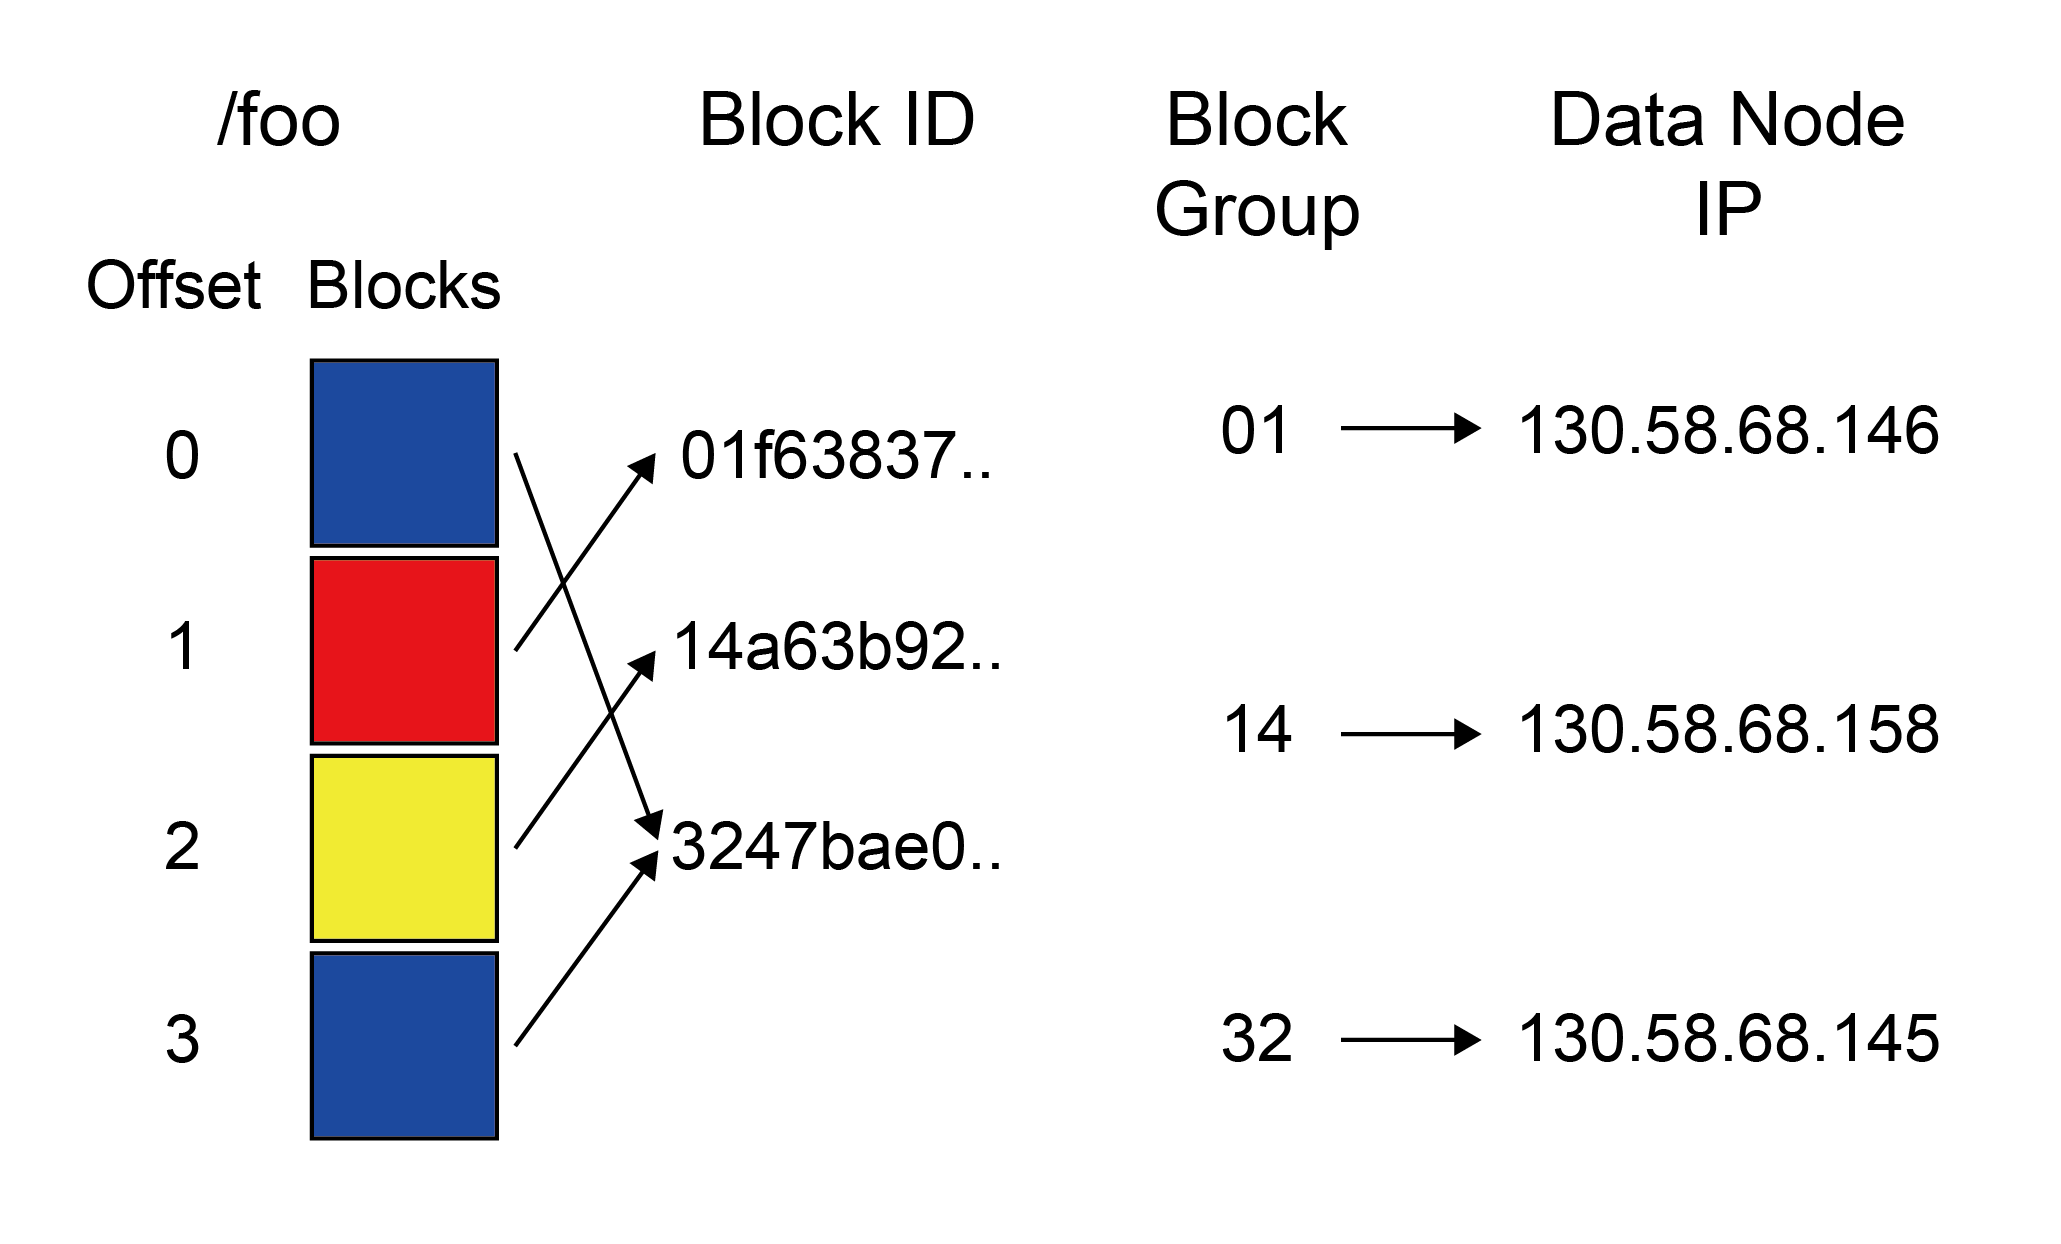
\includegraphics[width=0.75\textwidth]{metadata.png}
  \caption{{\label{metadata} }Reduct Metadata }
\end{figure*}

\subsection{Block Locations}\label{arch:block}
Each file is split into fixed-sized blocks, which are stored in the data nodes. Blocks are organized into block groups according to their block identifiers. Blocks of the same block group are stored in the same data node. Block groups are organized by the first two digits of their block identifier. Two blocks with identifiers that have the same first two digits belong to the same block group. Blocks are stored in the local file system of data nodes.  They are stored under a directory that corresponds to the first few digits of the block identifier. The initial assignment of a block group to a data node is random and no load balancing function is currently supported. 

\subsection{Consistency Model}\label{arch:cons}
Reduct follows a write-once, read-many model similar to the one used in HDFS. Hence, files in Reduct cannot be modified once written and closed. For simplicity, concurrent writes are not allowed and there may be only one writer writing to a file at a time. This greatly simplifies the consistency model as any operation on the file systems metadata is atomic. The file system guarantees that the first application to open a file in write mode is the only writer of that particular file. Other applications may concurrently read the file, however only up to the file offset the writer has updated. Atomic operation on the block map guarantees that concurrent write operations of a duplicate block do not cause any race conditions. The first application to create the block file in the local file system of a data node is the writer of that block.


\subsection{Deduplication}\label{arch:dedup}
Reduct supports deduplication by incorporating a block level fingerprinting index as part of its file system metadata and organizing block locations based on unique block identifiers which are generated by concatenating hash values computed on the block data with an offset. Hence, the granularity of the deduplication and that of the distributed file system are identical. The purpose of concatenating the hash value with the offset to block identifier is to avoid accidental collision that may corrupt data. If two blocks have the same hash value and data, only one copy is stored in a data node, and the two blocks are assigned the same block identifier. However, if two blocks have the same hash value, but different data, both copies are stored as separate files in the same data node and are assigned different block identifiers; the same hash value concatenated with different offsets. 

In addition to maintaining a fingerprinting index, the system performs byte-by-byte comparison to confirm that two blocks with the same hash value are identical. The block locations are organized in such a way that provides the locality that is crucial for executing byte-by-byte comparison without significantly compromising system performance. Further details about the deduplication process will be provided in Section~\ref{ops:write} of the paper. It is worth noting that our solution resolves the problem of having two separate metadata data structures by combining them into one.  Our solution solves the issue of data corruption due to hash collision by performing byte-by-byte comparisons.

\subsection{Limitations}\label{arch:slimit}
Compared to the scope of this project, the amount of time we had to complete this project was very limited. As a result, we focused on implementing deduplication and simplifying or omitting any aspect of the system that is not directly related to deduplication. Reduct only supports sequential, read, write, open, and close operations. At any level, the system is not fault tolerant as metadata is only stored in memory, data blocks are not replicated, and the master node does not take any action if a data node goes down. Reduct is very vulnerable to attacks as there is no authentication protocol or security measures. Other weaknesses include, but are not limited to, lack of checksum for data transfer and lack of load balancing. 

\begin{figure*}
  \center
  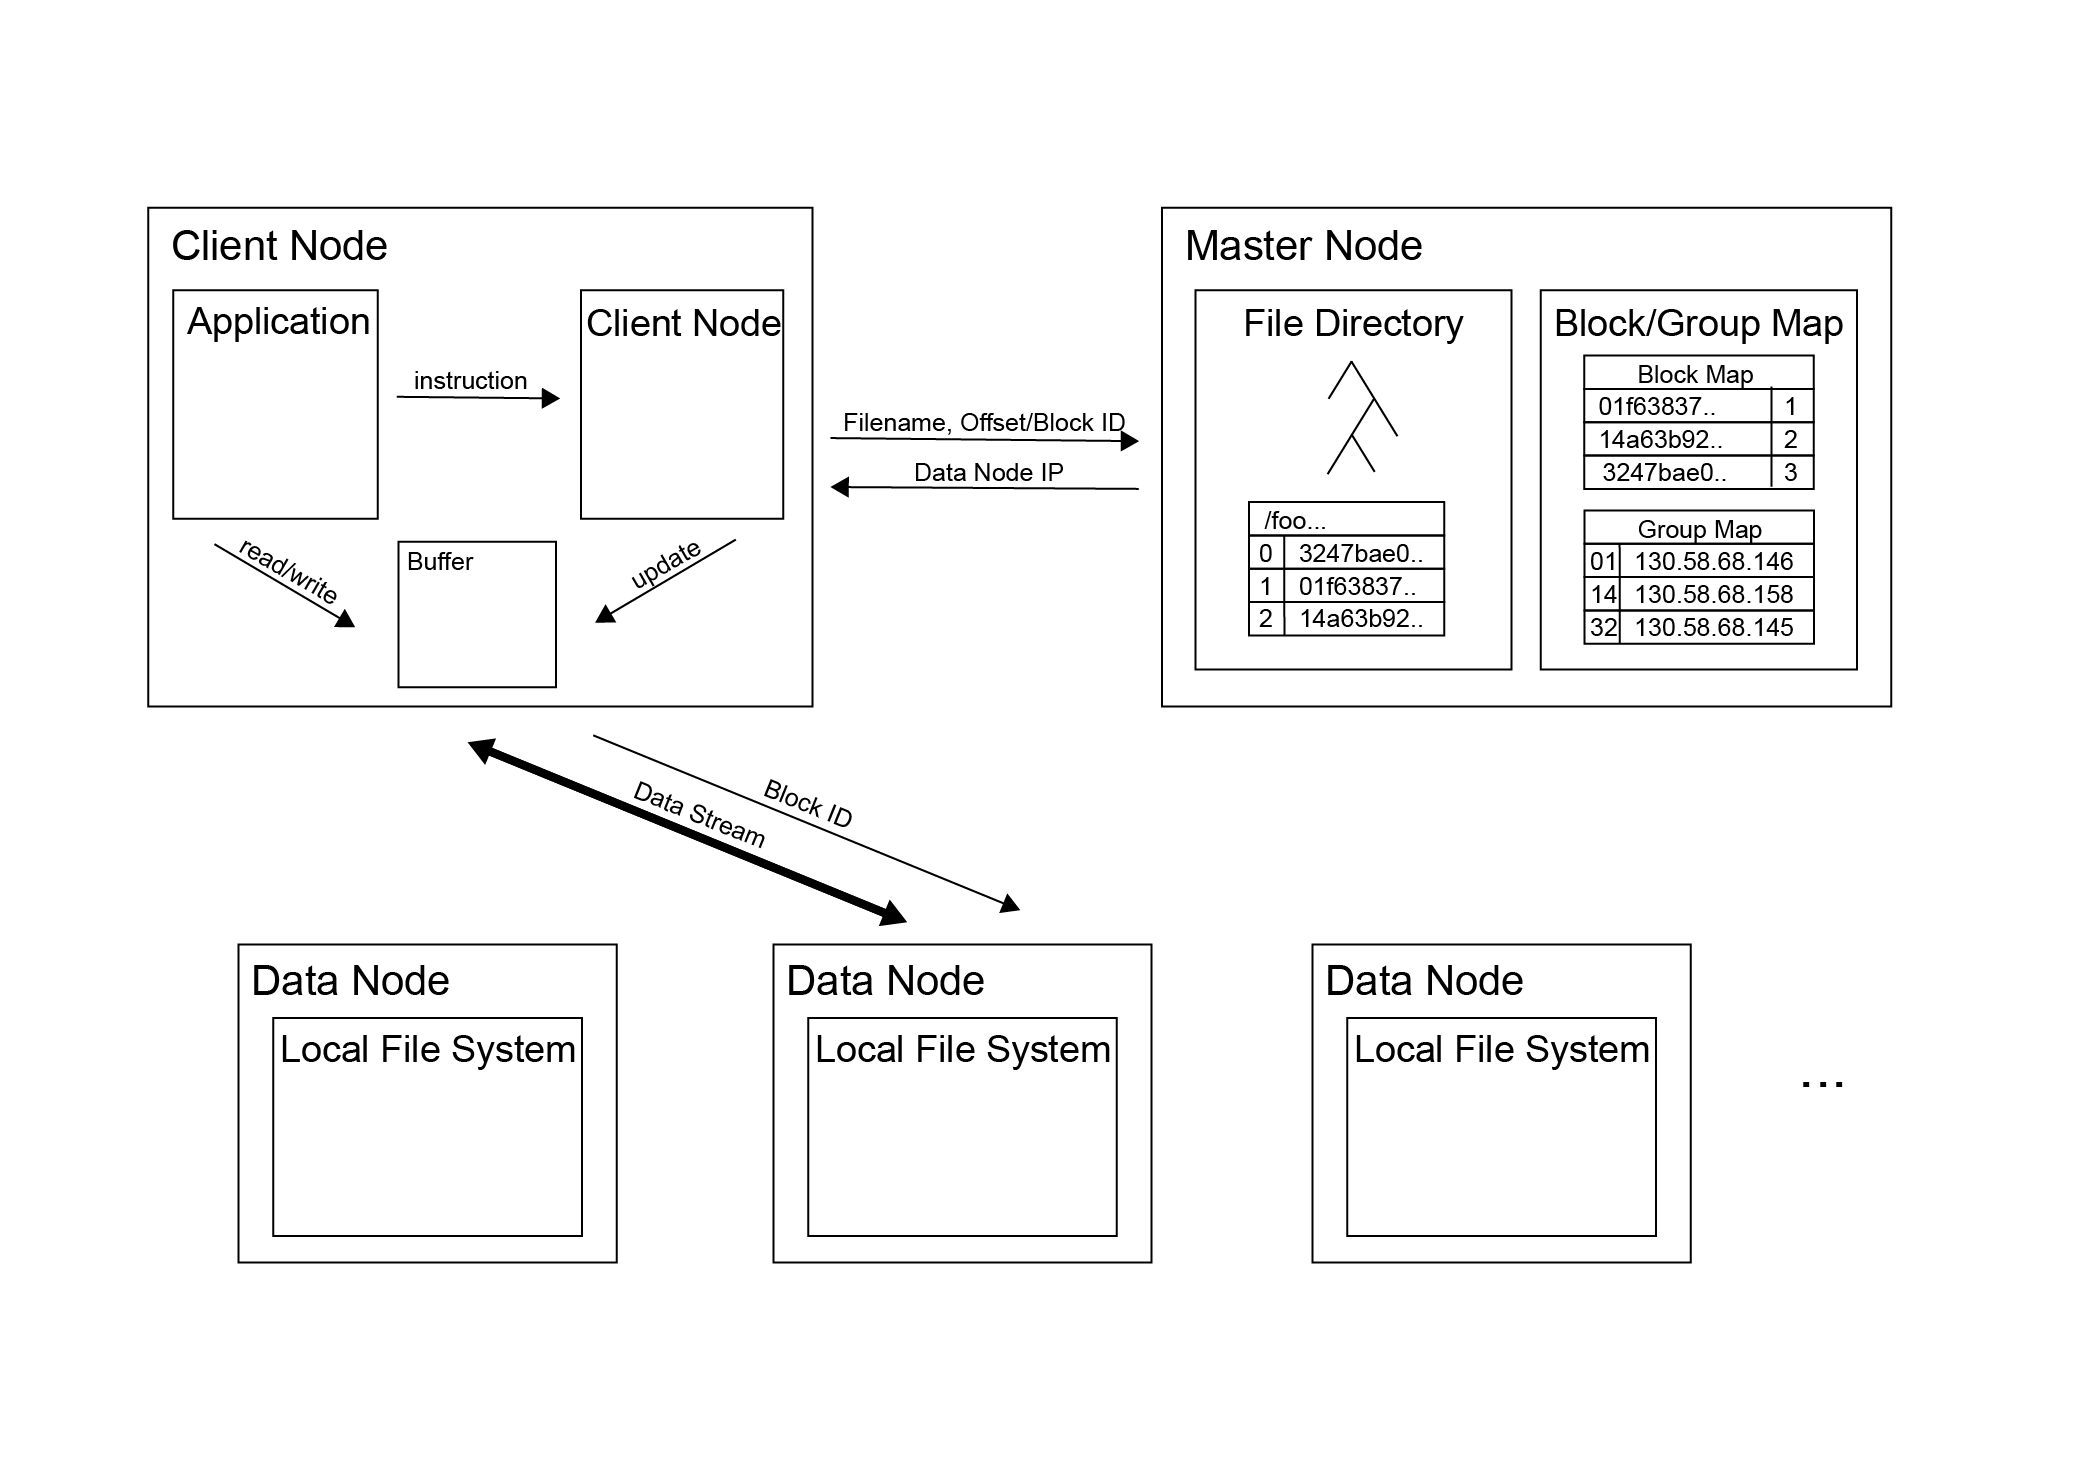
\includegraphics[width=1\textwidth]{overall.png}
  \caption{{\label{overall} }Reduct Architecture }
\end{figure*}

\section{Operations}\label{ops}

\subsection{Open}\label{ops:open}
When a client application opens a file, the ClientNode process sends the file name with an open tag (mode) to the master node. If the mode is in write and the file does not already exist, the master node adds a new file inode to the file directory and returns a complete message to the client node. The ClientNode process, then, initializes two shared buffers that the application can write data into. The application is provided a file handler identifier, which it can use to call the write operation. If the mode is read and the file already exists, the master node returns a complete message to the client node and the ClientNode process initializes a shared buffer for reading data from the data nodes. The application is provided with a file handler identifier, which may be used to call read operation on the file. In any other case, the operation fails and the master node returns an error message to the client node. A value of -1 is returned to the application. 

\subsection{Close}\label{ops:close}
If the file handler is in write mode, the client application requests the ClientNode process to upload the last block of data to the file system, following the process described in Section ~\ref{ops:write}, before closing the file. Then, the application sends a close message to the ClientNode process which sends the file name with a close tag to the master node. The master node returns a complete message and the shared buffers for reading/writing the file in the client node are deallocated.  


\subsection{Read}\label{ops:read}
When a client application reads a file, it reads from a data buffer of the block size. If it completes reading the buffer, it requests the ClientNode process to update the buffer. The ClientNode process sends the file name and file offset with a read tag to the master node. The master node checks if the file directory contains the file inode with the file name and the offset and retrieves the corresponding block identifier. Then, the master node checks the Group Map to retrieve the location of the block and returns the block identifier and the location. If the file is not found or the offset is outside the range, the master node returns an error message to the client node. After receiving the block identifier and the location, the client node establishes a TCP connection with the data node and sends the block identifier. If the block is in the local file system, the data node establishes a data stream and sends the block data, which is streamed into the buffer on the client node. If the block is not found, the data node sends an error message.  

\subsection{Write}\label{ops:write}
A file handler object in write mode has two data buffers of the block size. When a client application writes a file, it writes into one of the data buffers. Once it fills the buffer, it computes the hash value of the data block and generates a block identifier by concatenating the hash value with ``0." Then, it requests the ClientNode process to upload the data block to the file system. While the data block is being uploaded, the application continues writing into the second buffer. The ClientNode process sends the block identifier to the master node with a write tag. The master node then checks if the block identifier is already in BlockMap and if its block group is already in GroupMap. If the block identifier is not in BlockMap, it adds a key value pair of the block identifier and 0. If the block group is not in GroupMap, it randomly assigns the block group to a data node and adds a key value pair of the block group and the data node location to GroupMap. Then it returns the data node location to the client node. ClientNode establishes TCP connection with the right data node and sends the block identifier with a write tag. Then, it sends the data block to the data node.

If a data block of the given block identifier does not already exist in the local file system, the data node creates a new file under the appropriate directory and writes the data block into the file. Then, it sends a complete message to the client node. The client node then sends the file name, offset, and block identifier to the master node.  The master node then updates the metadata by adding a new entry to the block identifier table of the file inode and incrementing the number of duplicates of the block in BlockMap. Finally, it sends a complete message to the client node.       

If a data block of the given block identifier already exists in the local file system, the data node performs a byte-by-byte comparison between the data received from the client node and the data stored in the data block file. If the data block is indeed a duplicate, the data node sends a message to the client node that the data block is a duplicate. Then, the client node sends the file name, offset, and block identifier to the master node, which follows the aforementioned process to update the metadata. If the data block is not a duplicate, the data node sends a message specifying that it is not a duplicate to the client node. The client node generates a new block identifier by incriminating the last character of the identifier and tries writing the block again with the new block identifier, following the procedure described above. 

\section {Results}\label{results}

\subsection{Method}\label{results:method}
Several experiments were conducted to measure the performance of our system. For all of the experiments, one master node, four client nodes, and four data nodes were used. Each machine had configurations of 3.40 GHz i7-6700 quad core processor, 31 GB of RAM, 256GB TLC NAND solid state drive, and 1 Gbps Ethernet connection. The SHA-1 algorithm was used as our cryptographic hash function. Each experiment consisted of measuring the time it took for each client to simultaneously write its own set of files into the file system and to simultaneously read it. The deduplication ratio was also measured for each experiment. In the first two experiments, each client wrote and read 256 MB of data while in the third experiment, each client wrote and read about 250 MB of data with some variations among different clients.

Scripts were used to execute applications for the experiments. Different block sizes were tested for each experiment. In the first experiment, each client wrote and read one file consisting of an array of one repeated character. The repeated character was different for each client. In the second experiment, each client wrote and read one file that consists of an array of randomly generated characters. In the third experiment, each client wrote and read several files with sizes ranging from 13 to 151 MB. 34.57\% of the total set of files in the third experiment were duplicates at file level.

\subsection{Deduplication}\label{results:deduplication}
In the first experiment, duplication ratio decreased with increasing block size as shown in Table~\ref{dedupresults}. There were no duplicates in the second experiment, while the ratio was 1.53:1 across different block sizes in the third experiment. The results from the first experiments imply that deduplication improves with smaller block size. The results from the second and third experiments, however, suggest that if there is no duplicate or duplicates exist only at file level, there is no additional advantage to using a smaller block size.

\begin{table}[H]
\begin{center}
\begin{center}
\begin{tabular}{ |c|c|c|c|c|c| } 
\hline
Block(MB) & 1 & 2 & 4 & 8 & 16 \\
\hline
Ratio & 256:1 & 128:1 & 64:1 & 32:1 & 16:1\\
\hline
\end{tabular}
\end{center}

\caption{\label{dedupresults} Deduplication ratios for different block sizes in Experiment 1}
\end{center}
\end{table}

\subsection{Read}\label{results:read}
The read speed per client was computed based on runtime for different block sizes in each experiment. In all three experiments, read speed increased with increasing block size as the communication cost per byte decreased, as shown in Figure~\ref{read_speed}. The maximum speed measured was 36.13 MB/s for block size of 16MB in the second experiment while the minimum speed measured was 7.65MB/s for the block size of 1MB in the third experiment. Read speeds were slightly faster in the second experiment than those in the first experiment. The read speeds in the third experiment were slower than those in the other two. This is likely due to the fact that there were extra communication costs for opening and closing multiple files as opposed to just one file.

\begin{figure}[H]
  \center
  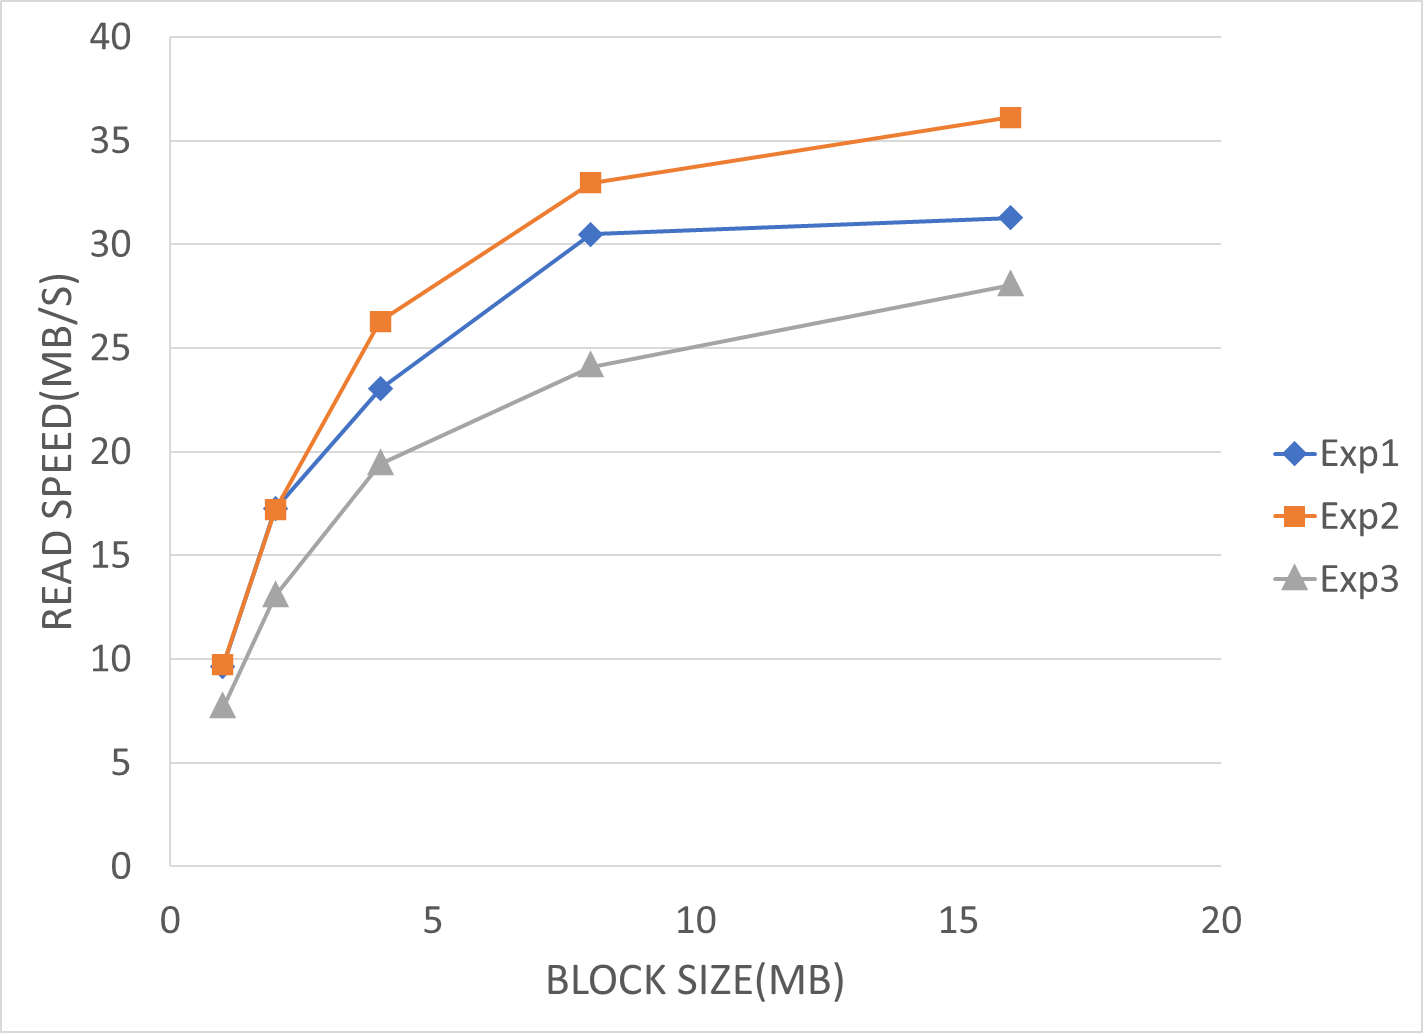
\includegraphics[width=0.48\textwidth]{read_speed.png}
  \caption{{\label{read_speed} }Read speed(MB/s) for different block sizes in Experiment 1,2, and 3 }
\end{figure}

\subsection{Write}\label{results:write}
Similarly, write speed per client was computed for different block sizes in each experiment. In all three experiments, write speed increased with increasing block size as shown in Figure~\ref{write_speed}. The maximum write speed measured was 36.15MB/s for block size of 16MB in the first experiment. The minimum speed measured was 3.69MB/s for block size of 1Mb in the third experiment. As shown in Figure~\ref{write_speed}, the write speeds were fastest in the first experiment, followed by the third experiment and finally the second experiment. It is worth noting that this is precisely the order of the deduplication ratio; the higher the ratio, the faster the write speed. For any duplicate block, the write operation consists of reading the block of data that is already stored and performing a byte-by-byte comparison. As disk read speed is significantly faster than disk write speed, the operation is faster than writing a new block of data into the local disk of a data node. Furthermore, there is no extra cost for detecting and locating a duplicate data block as block locations are assigned based on the hash value of each data block. Consequently, higher deduplication ratio results in faster write speed, as observed in the experiments. In extreme cases where most of the data are duplicates like in the first experiment, most write operations involve reading from the disk, instead of writing into it. In fact, the maximum write speed was faster than the maximum read speed.

\begin{figure}[H]
  \center
  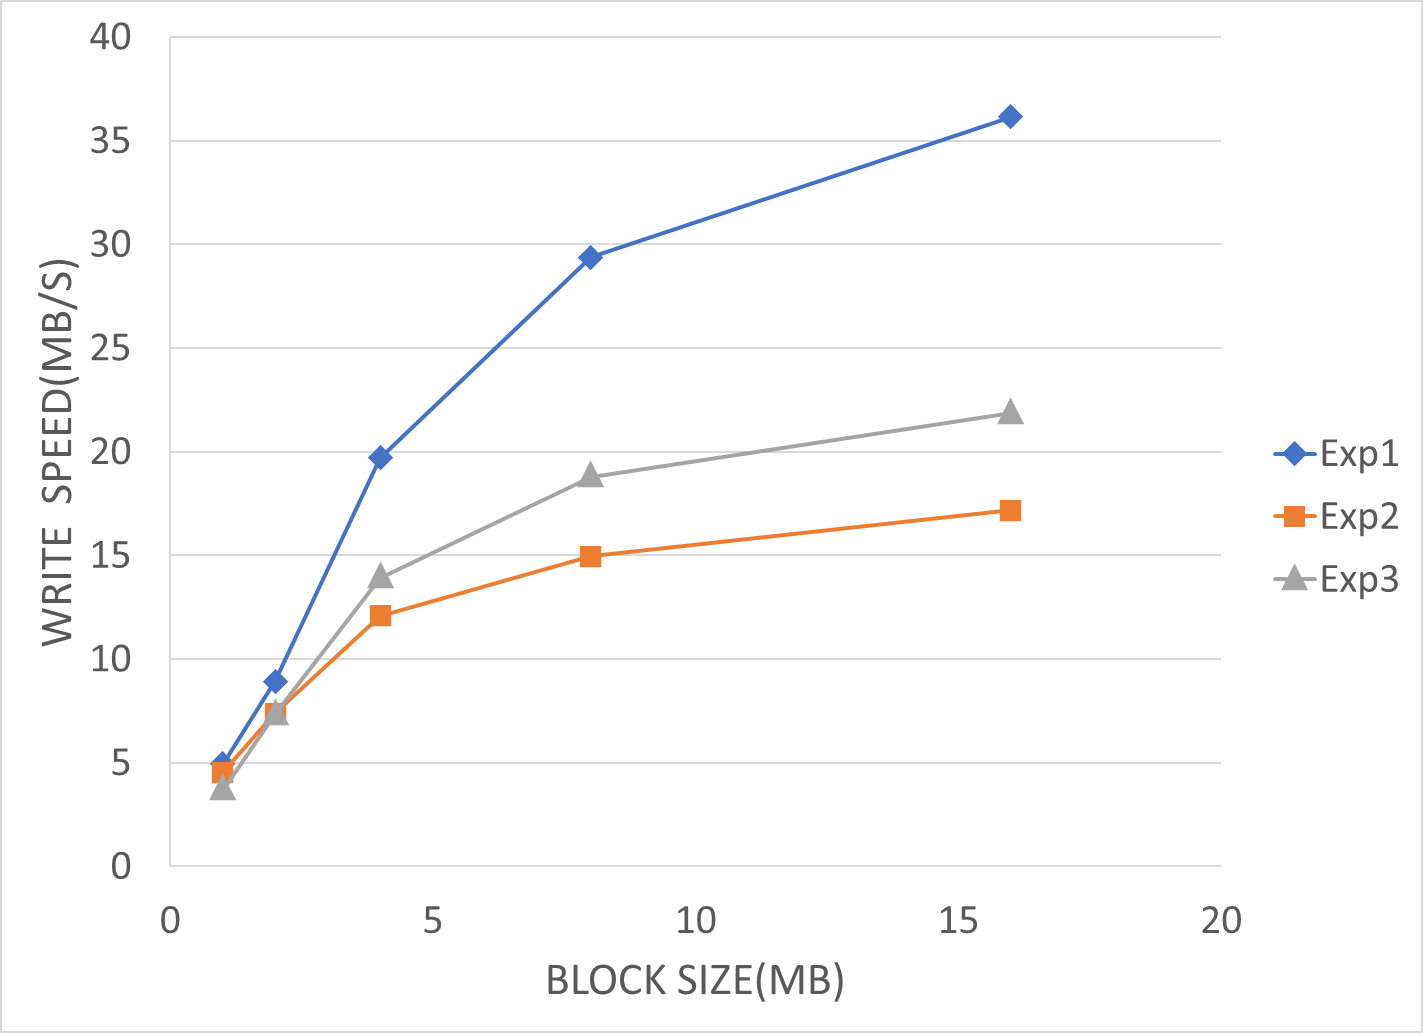
\includegraphics[width=0.48\textwidth]{write_speed.png}
  \caption{{\label{write_speed} }Write speed(MB/s) for different block sizes in Experiment 1,2, and 3 }
\end{figure}

\subsection{Implications}\label{result:deduplication}
The relationship between block size, read/write speeds, and deduplication ratio suggests that there is a trade off between performance and deduplication. Smaller block sizes provide a finer granularity for detecting duplicates at sub-file level and allow more deduplication. However, smaller block sizes also increase communication overhead per byte of data, and thus result in slower read/write speed. The relationship, however, is highly dependent on the nature of the data as illustrated by the results of the latter two experiments. In cases where there are only duplicates at file level or there are no duplicates, smaller block size significantly compromises the read/write speed without any additional benefit. A study by Dutch and Bolosky revealed that most duplicates occur at file level, not sub-file level\cite{microsoft}. Also, given that files typically stored in a distributed file system are large and read/write throughput is very important for performance of typical applications executed on a distributed file system, it seems reasonable to use large block sizes comparable to the default size used by the Google File System or HDFS. 

The main purpose of the experiments was to measure the overall performance of Reduct, especially with regards to how much systematic overhead deduplication adds. There are two major sources of extra overhead. The first is computing the hash value of a data block. The second is performing byte-by-byte comparison between two data blocks that have the same hash value. The direct impact of each respective operation on runtime was not measured due to time constraint.  However, the impact can be inferred from a comparison between the different experimental results. For example, read and write operations in the first experiment are almost identical as they involve reading blocks of data, except that the write operation involves extra operations of computing hash values and performing byte-by-byte comparison. 

Even considering that less optimization was implemented for the read operation, the fact that write speed is almost as fast as read speed (faster in case of the maximum speed) suggests that hash computation and byte-by-byte comparison do not compromise performance significantly. A comparison between results from the first two experiments reveals that data deduplication could even improve write speed. In the first experiment, every operation involves byte-by-byte comparison as every block is a duplicate.  In the second experiment, there is no byte-by-byte comparison as there is no duplicate block. We see that write speeds in the first experiment are significantly faster than those in the second experiment. This suggests that the detection of duplicates by a byte-by-byte comparison is at least as fast as writing a new block of data, if not faster.

\section{Conclusions and Future Directions}\label{conc}
Due to significant time constraints, there were certain limitations to the project in terms of system implementation and experimental results. Despite this, we found compelling results with significant implications. The main goal of the project was to design, implement, and test a novel distributed file system model that supports data deduplication without the issues other existing systems have. Other than deduplication, the primary focus of the research was investigating how deduplication affects the performance of the system. Our system addresses issues inherent to the solution with two sets of metadata by combining these distinct sets into one and utilizing it as both the file system metadata and fingerprinting index. The system also avoids data corruption due to hash collision by performing byte-by-byte comparisons. 

Regarding the feasibility of this model, the experimental results are rather promising. The results suggest not only that deduplication adds minimal communication overhead, but also that it could improve performance under some circumstances. Unfortunately, the system we implemented was not highly optimized due to time constraint, but our model is quite flexible in terms of implementation details. For example, a block identifier, which is a 40 character long hexadecimal string, is significantly longer than the identifier used by any typical block-based distributed file system. It is possible to decrease the amount of metadata per unit of file data by using shorter identifiers as the system reliably handles accidental hash collisions. Another related example is that it is possible to use weaker, but reasonably strong hash functions that might have better runtime to improve performance. Load balancing is a function that we did not implement, but considered when we designed the system. Specifically, we organized blocks into block groups so a group could serve as a unit for transferring data between different nodes. The granularity of the group could be configured appropriately to meet specific needs.     

One must be careful about extrapolating results from this paper as the system we implemented is far simpler and more vulnerable than full scale systems that are already in use. Also, we did not test our system using any standardized benchmark test. The experimental results, however, suggest that our model is worth investigating in future research. The primary goal of the future research would be to design and implement a full scale distributed file system that is far more robust and reliable. It could incorporate features of conventional distributed file systems, including, but not limited to, maintenance of log files of metadata, replication of data blocks, authentication protocol, and security measures. The system could then be tested for performance, taking the additional variables into account. 

\section{Meta-discussion}\label{meta} 
Our time constraint was one of the biggest challenges of this project. We were also challenged by various difficulties due to COVID-19. Not being able to occupy the same physical space in the same zone made communication and coordination amongst the team members as well as with our instructor more challenging. Nonetheless, we maintained our original plan to design and implement our own system. The most important task was to simplify the model, making the entire project feasible within the given time period. Even after spending a significant amount of time carefully planning and simplifying our model, we found that there were many details that we had to work out as we built the system.

Another major challenge was learning how to use the various tools needed to implement our ideas. This was the first time we conducted a project of this size using C++, so learning how to use tools, including TCP socket programming, shared memory, openssl, Makefile, multithreading, and object oriented programming was quite challenging. We checked various resources on the internet, referred to past work in other computer science courses, and asked for help when necessary and eventually learned how to use them.

Lastly, debugging was extremely difficult as it is a distributed system. Even conducting incremental testing was not easy given that every component was tightly interconnected. So even if a component seemed sound, bugs unexpectedly arose as we implemented additional components of the system. We resorted to execution of numerous sample programs, and debug print statements to locate and fix bugs. 

Overall, our achievement did not deviate too much from our original proposal. When we were planning out our project, we tried to be as realistic as possible and suggested any additional plan only as a possibility. We are very pleased that we completed the project in time despite extraordinary circumstances. 

\section{Acknowledgement}\label{ackn}
We would like to thank Professor Newhall for the advice and guidance she provided us throughout the project. We would also like to acknowledge Professor Knerr for providing machine configuration information necessary for conducting experiments. 

\bibliography{finalreport}
\bibliographystyle{plain}



\end{document}
